%!TEX program = xelatex
%%%%%%%%%%%%%%%%%%%%%%%%%%%%%%%%%%%%%%%%%
% Short Sectioned Assignment
% LaTeX Template
% Version 1.0 (5/5/12)
%
% This template has been downloaded from:
% http://www.LaTeXTemplates.com
%
% Original author:
% Frits Wenneker (http://www.howtotex.com)
%
% License:
% CC BY-NC-SA 3.0 (http://creativecommons.org/licenses/by-nc-sa/3.0/)
%
%%%%%%%%%%%%%%%%%%%%%%%%%%%%%%%%%%%%%%%%%

%----------------------------------------------------------------------------------------
%	PACKAGES AND OTHER DOCUMENT CONFIGURATIONS
%----------------------------------------------------------------------------------------

\documentclass[paper=a4, fontsize=11pt]{scrartcl} % A4 paper and 11pt font size
\usepackage{xeCJK}
\usepackage[T1]{fontenc} % Use 8-bit encoding that has 256 glyphs
\usepackage{fourier} % Use the Adobe Utopia font for the document - comment this line to return to the LaTeX default
\usepackage[english]{babel} % English language/hyphenation
\usepackage{amsmath,amsfonts,amsthm} % Math packages
\usepackage{lipsum} % Used for inserting dummy 'Lorem ipsum' text into the template
\usepackage{enumerate}
\usepackage{sectsty} % Allows customizing section commands
\usepackage{caption}
\allsectionsfont{\normalfont\scshape} % Make all sections centered, the default font and small caps

\usepackage{fancyhdr} % Custom headers and footers
\pagestyle{fancyplain} % Makes all pages in the document conform to the custom headers and footers
\fancyhead{} % No page header - if you want one, create it in the same way as the footers below
\fancyfoot[L]{} % Empty left footer
\fancyfoot[C]{} % Empty center footer
\fancyfoot[R]{\thepage} % Page numbering for right footer
\renewcommand{\headrulewidth}{0pt} % Remove header underlines
\renewcommand{\footrulewidth}{0pt} % Remove footer underlines
\setlength{\headheight}{13.6pt} % Customize the height of the header

%\numberwithin{equation}{section} % Number equations within sections (i.e. 1.1, 1.2, 2.1, 2.2 instead of 1, 2, 3, 4)
\numberwithin{figure}{section} % Number figures within sections (i.e. 1.1, 1.2, 2.1, 2.2 instead of 1, 2, 3, 4)
\numberwithin{table}{section} % Number tables within sections (i.e. 1.1, 1.2, 2.1, 2.2 instead of 1, 2, 3, 4)

\setlength\parindent{0pt} % Removes all indentation from paragraphs - comment this line for an assignment with lots of text

\usepackage{bm}
\usepackage{algorithm}
\usepackage{algorithmic}

%----------------------------------------------------------------------------------------
%	TITLE SECTION
%----------------------------------------------------------------------------------------

\newcommand{\horrule}[1]{\rule{\linewidth}{#1}} % Create horizontal rule command with 1 argument of height

\title{	
\normalfont \normalsize 
\textsc{Zhiyuan College, Shanghai Jiao Tong University} \\ % Your university, school and/or department name(s)
\horrule{0.5pt} \\[0.4cm] % Thin top horizontal rule
\huge CS 225: Probability and Computing Homework Final \\ % The assignment title
\horrule{2pt} \\ % Thick bottom horizontal rule
}

\author{
\normalsize
	Zihao Ye
} % Your name

\date{\normalsize\today} % Today's date or a custom date

\newtheorem{claim}{Claim}

\begin{document}

\maketitle % Print the title

\section*{Problem 1}
考虑概率方法.

假设$S$为有$n$个节点, $m$条边的不含$H$的图, 则由题意, 在完全图$G$中将$S$中所有的边染成一种颜色, 不会出现同色的子图$H$.

现在进行如下操作:
\begin{itemize}
	\item 枚举颜色$i$.
	\item 在$G$中随机sample $S$的一个同构子图$S_i$, 将它染成颜色$c_i$(不管它之前是否被染色过).
\end{itemize}

定义随机变量$X_e$:

$$X_e = \left\{ 
\begin{array}{ll}
0 & e \textrm{ has been colored during the algorithm.} \\
1 & e \textrm{ hasn't been colored during the algorithm.} 
\end{array}
\right. $$

令$X = \sum\limits_{e\in E} X_e$, 则

$$E[X] = {n\choose2}\left(1-\frac{m}{{n\choose 2}}\right)^k \leq {n\choose 2}e^{-2\log n} \leq \frac{1}{2} < 1$$

因此存在一个outcome使得$X = 0$, 即所有边都被染色且不存在同色的子图$H$.

\section*{Problem 2}
\begin{enumerate}[(a)]
	\item 
	$$E[X_{np}] = {n\choose 3}p^3 $$

	设$X_{np}^{(t)}$为三角形$t$的三条边是否都被选, 可以证明$\left\{X_{np}^{(t)}\right\}$之间pairwisely independent.

	因此$$\textit{Var}\left[X_{np}\right] = {n\choose 3}\textit{Var}\left[X_{np}^{(t)}\right] = {n\choose 3}p^3(1-p^3)$$.

	由\textit{Chebyshev Inequality}可以得到:

	$$\textit{Pr}\left[\left|X_{np} - {n\choose 3}p^3\right|\geq t\right] \leq \frac{{n\choose 3}p^3(1-p^3)}{t^2}$$

	下面考虑使用\textit{Martingale}得到的界:

	令$X_i$为$e_i$是否被选, $f(\mathbf{X})$为三角形的个数 , 则:
	$$Y_i = E\left[f(X_1, \cdots, X_n) \mid X_1, \cdots, X_i \right]$$

	是一个\textit{Doob Sequence}, 且满足条件
	$$\left|Y_k - Y_{k-1}\right| \leq n - 2 $$

	由\textit{Azuma's Inequality}得:

	$$Pr\left[\left|f(\mathbf{X}) - E\left[f(\mathbf{X})\right]\right| \geq t\right]\leq 2 \exp\left(-\frac{t^2}{n(n-1)(n-2)^2}\right) $$
\end{enumerate}
\section*{Problem 3}
	由之前对sample matching的分析, 证明\textit{rapidly mixing}的关键在于证明

	\[
		\max_{M,M'}\frac{2m
		\left| \left\{
		(I,F) \mid (M,M')\in \gamma_{IF}
		\right\} \right|
		}{|\Omega|} \in \textit{poly}(n) \in \left(\log |\Omega|\right)^{O(1)}
	\]	
	
	之前允许\textit{edge exchange}的情况下, 通过特别地构造\textit{Canonical Path}, 证明了$$\left| \left\{
		(I,F) \mid (M,M')\in \gamma_{IF}
		\right\} \right|= O(|\Omega|)$$
	
	下面令$\left| \left\{
		(I,F) \mid (M,M')\in \gamma_{IF}
		\right\} \right|$为$P_{IF}$.

	现在证明即使只允许\textit{edge addition}和\textit{edge deletion}的情况下, $P_{IF}$仍然是$O(|\Omega|)$.

	在之前的证明中使用了\textit{encoding}的方法, 在这里我们仿照这一方法.

	对于每个$I$和$F$, 将所有$I\bigoplus F$的\textit{path}和\textit{loop}编号, 并给每个path和loop中的边编号(path从顶点开始, loop从任意一个点开始).

	对于\textit{loop}和\textit{path}, 分别按如下的\textit{Canonical Path}进行transition. 
	\begin{figure}[H]
	\centering
	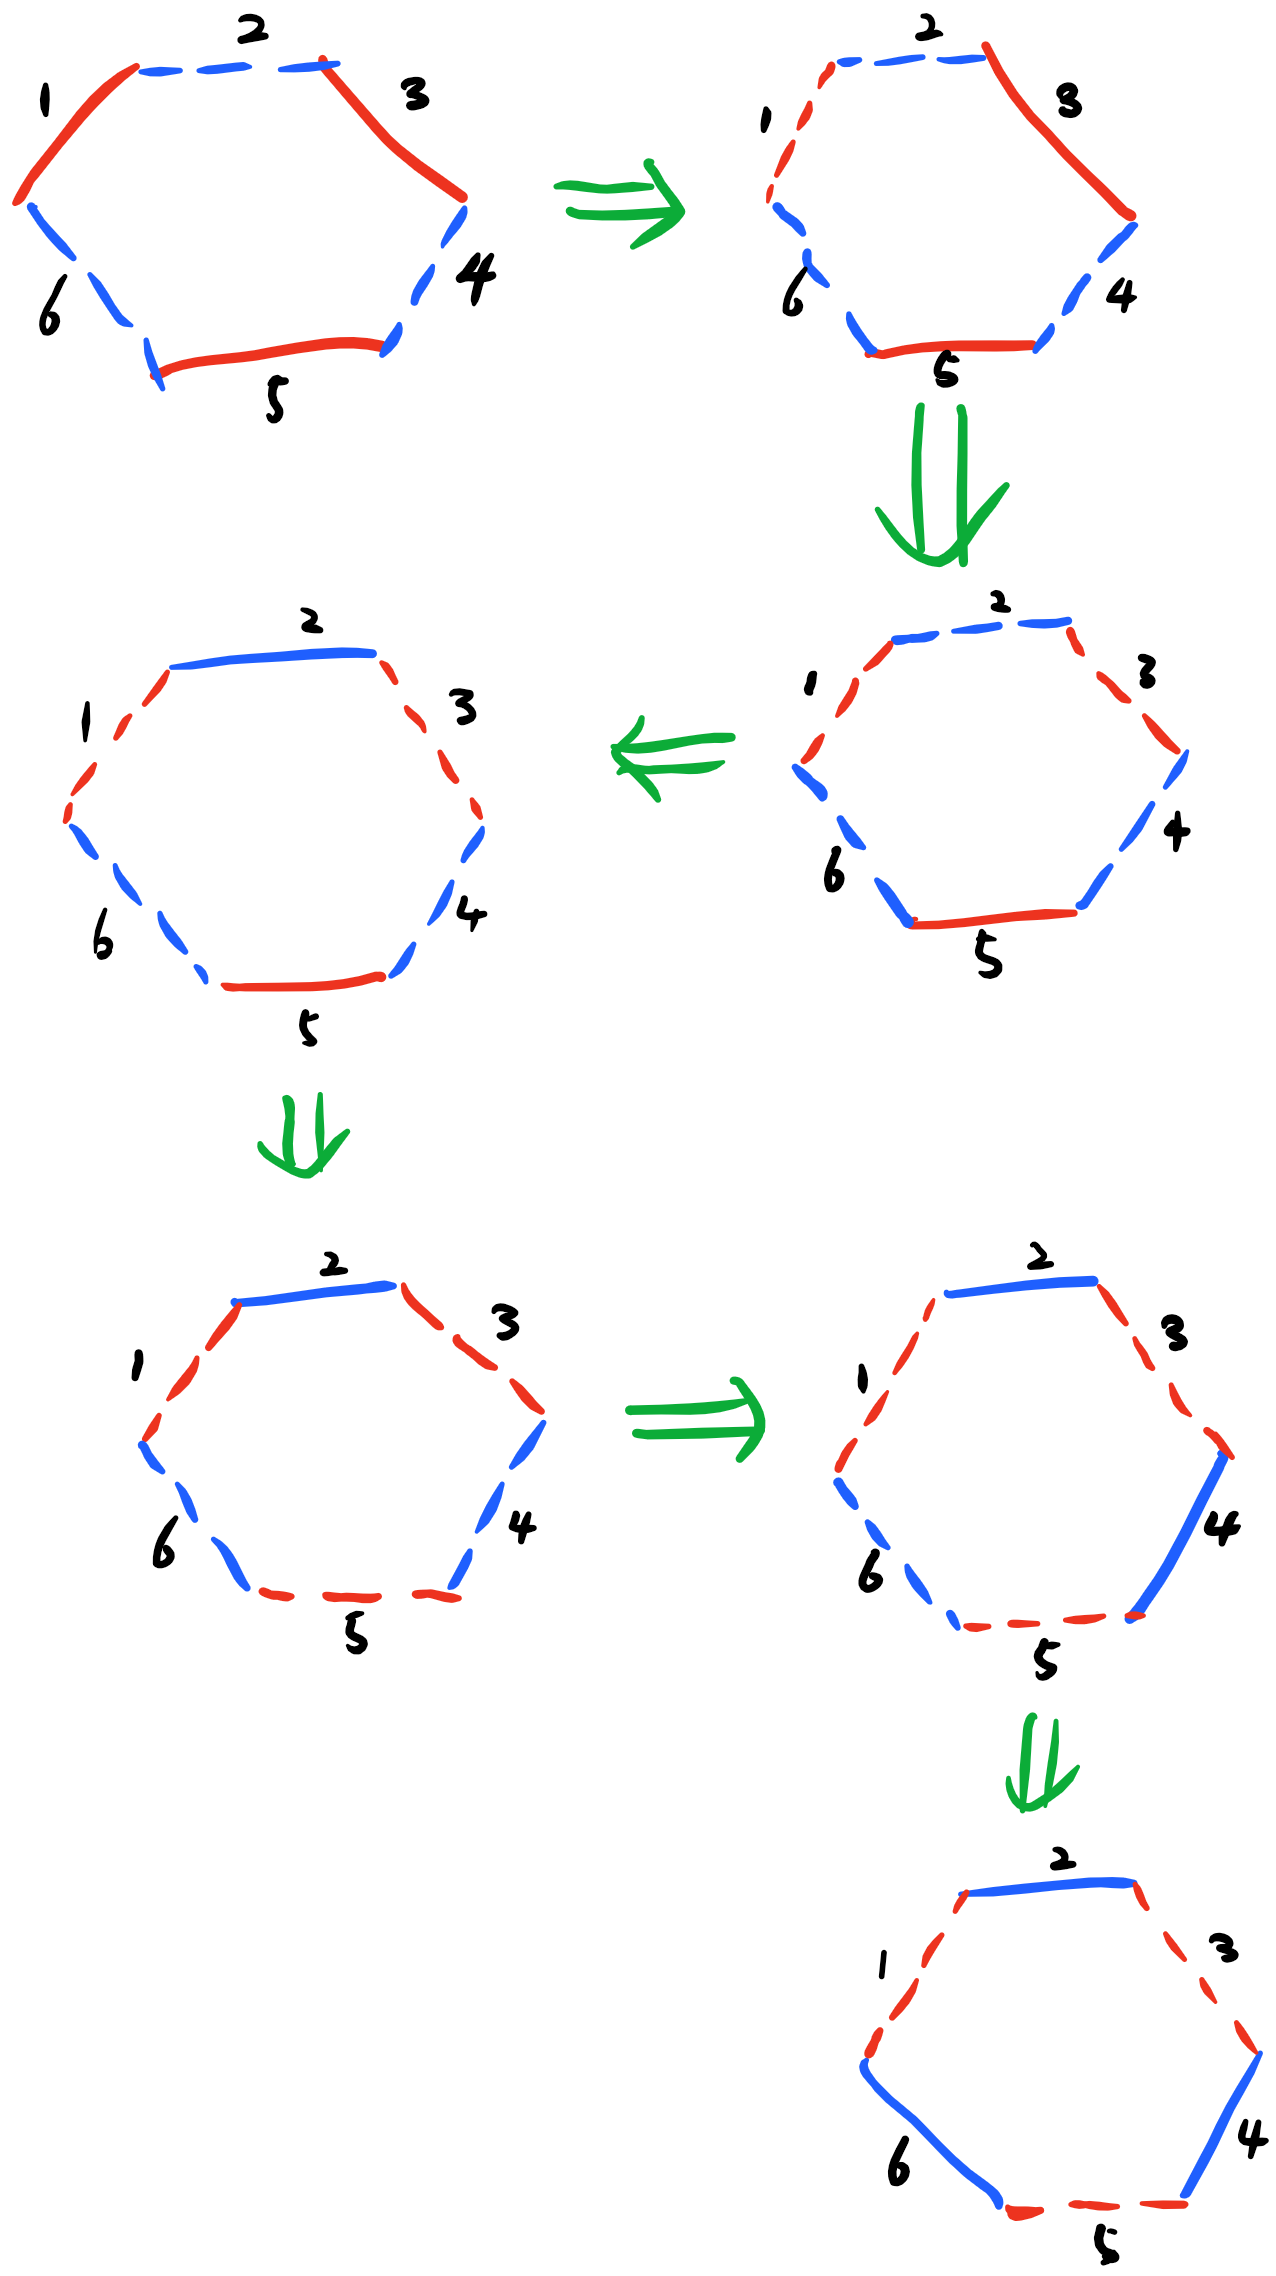
\includegraphics[width=300pt]{pic2.png}
	\caption*{loop}
	\end{figure}

	\begin{figure}[H]
	\centering
	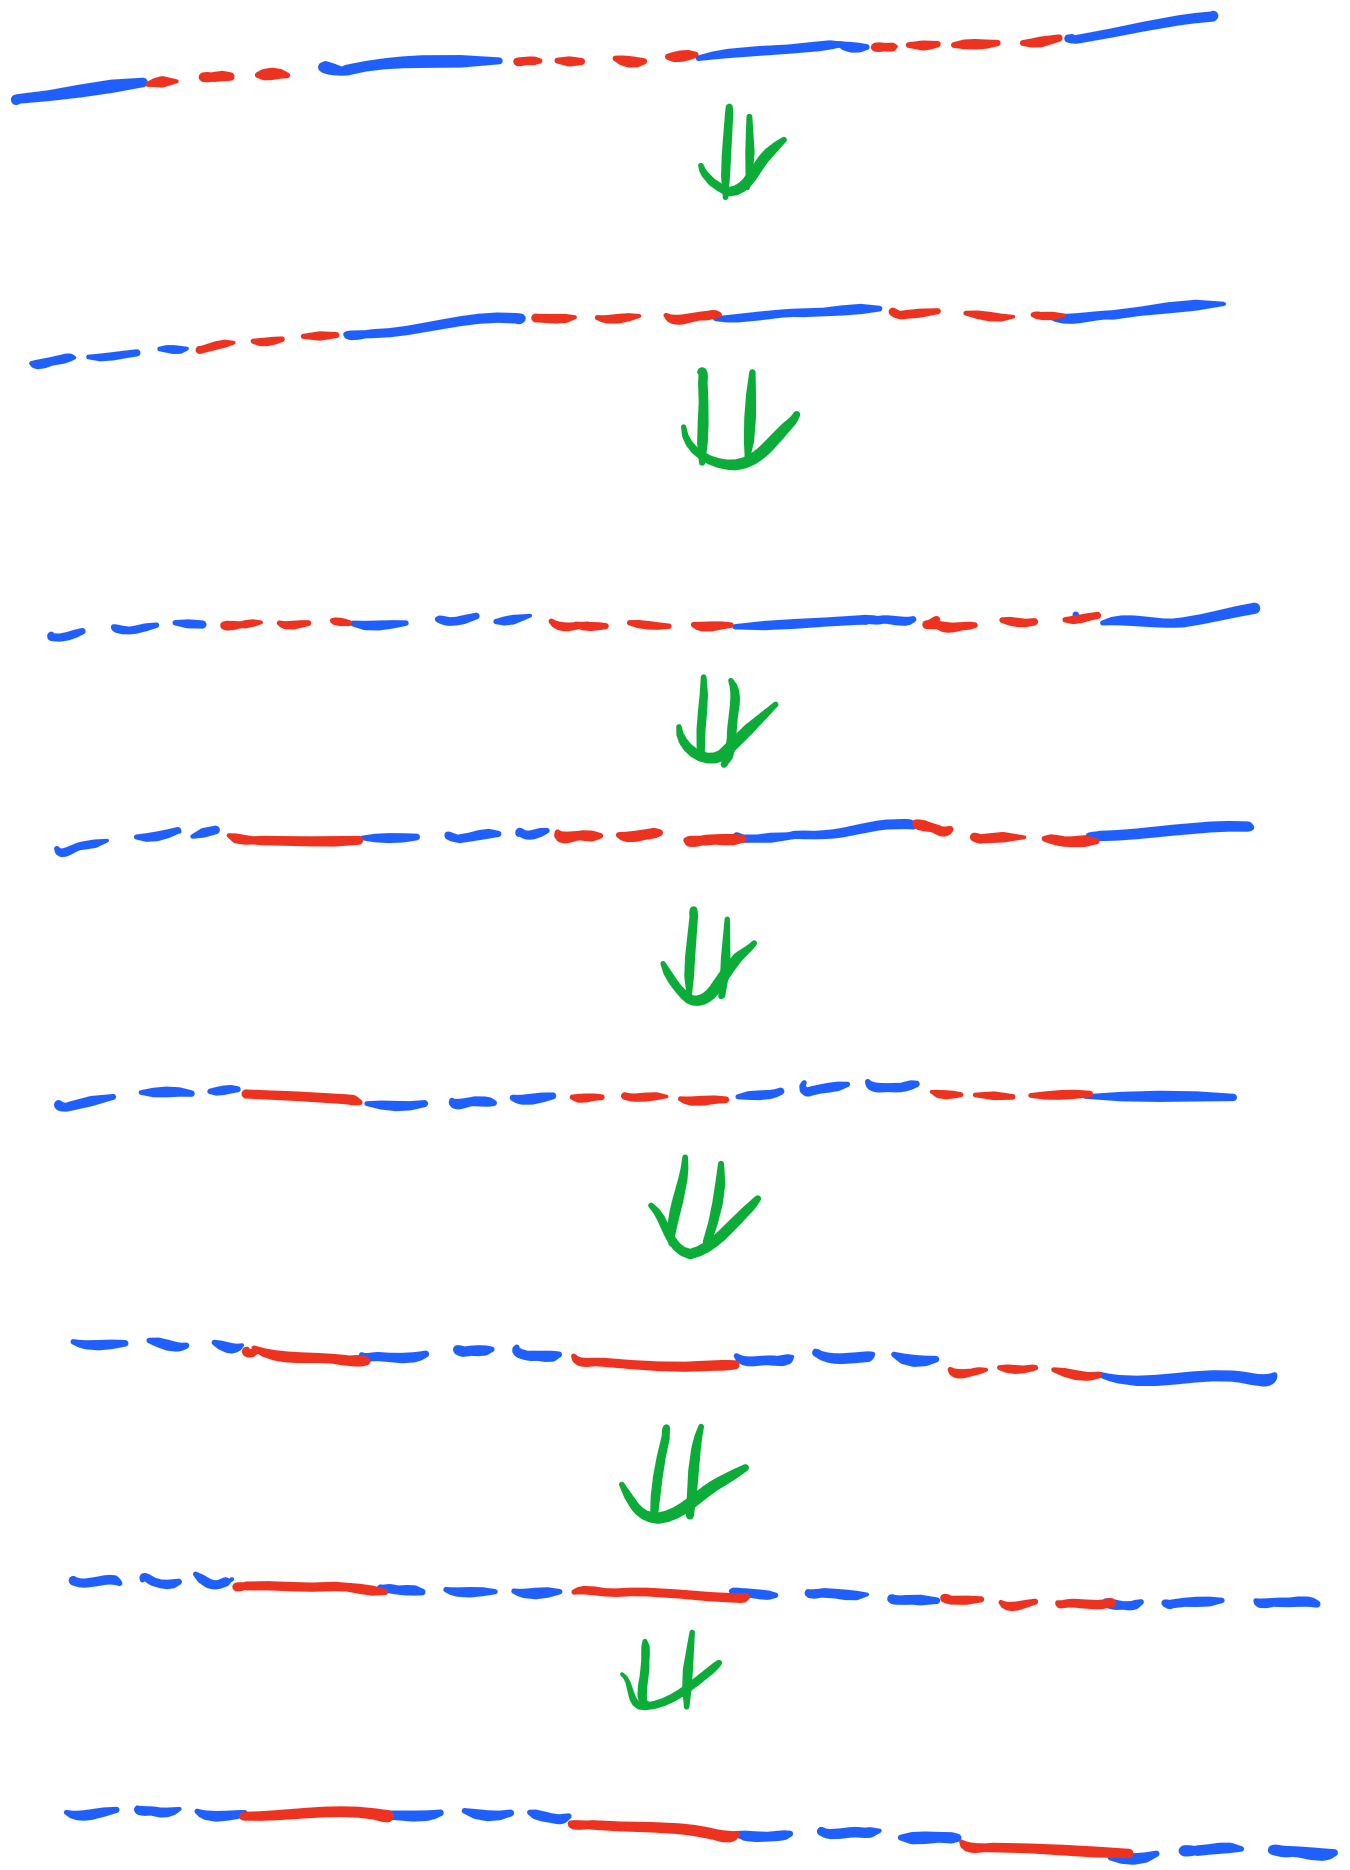
\includegraphics[width=300pt]{pic3.png}
	\caption*{path}
	\end{figure}

	为了计算$P_{IF}$, 在给定$(M, M')$的情况下, 我们需要找到一个从$(I, F)$到matching的映射(因为我们希望$P_{IF}=poly(n)\times|\Omega|$).

	事实上$I\bigoplus F - (M\bigcup M')$并不是一个matching: 如下图:
	
	\begin{figure}[H]
	\centering
	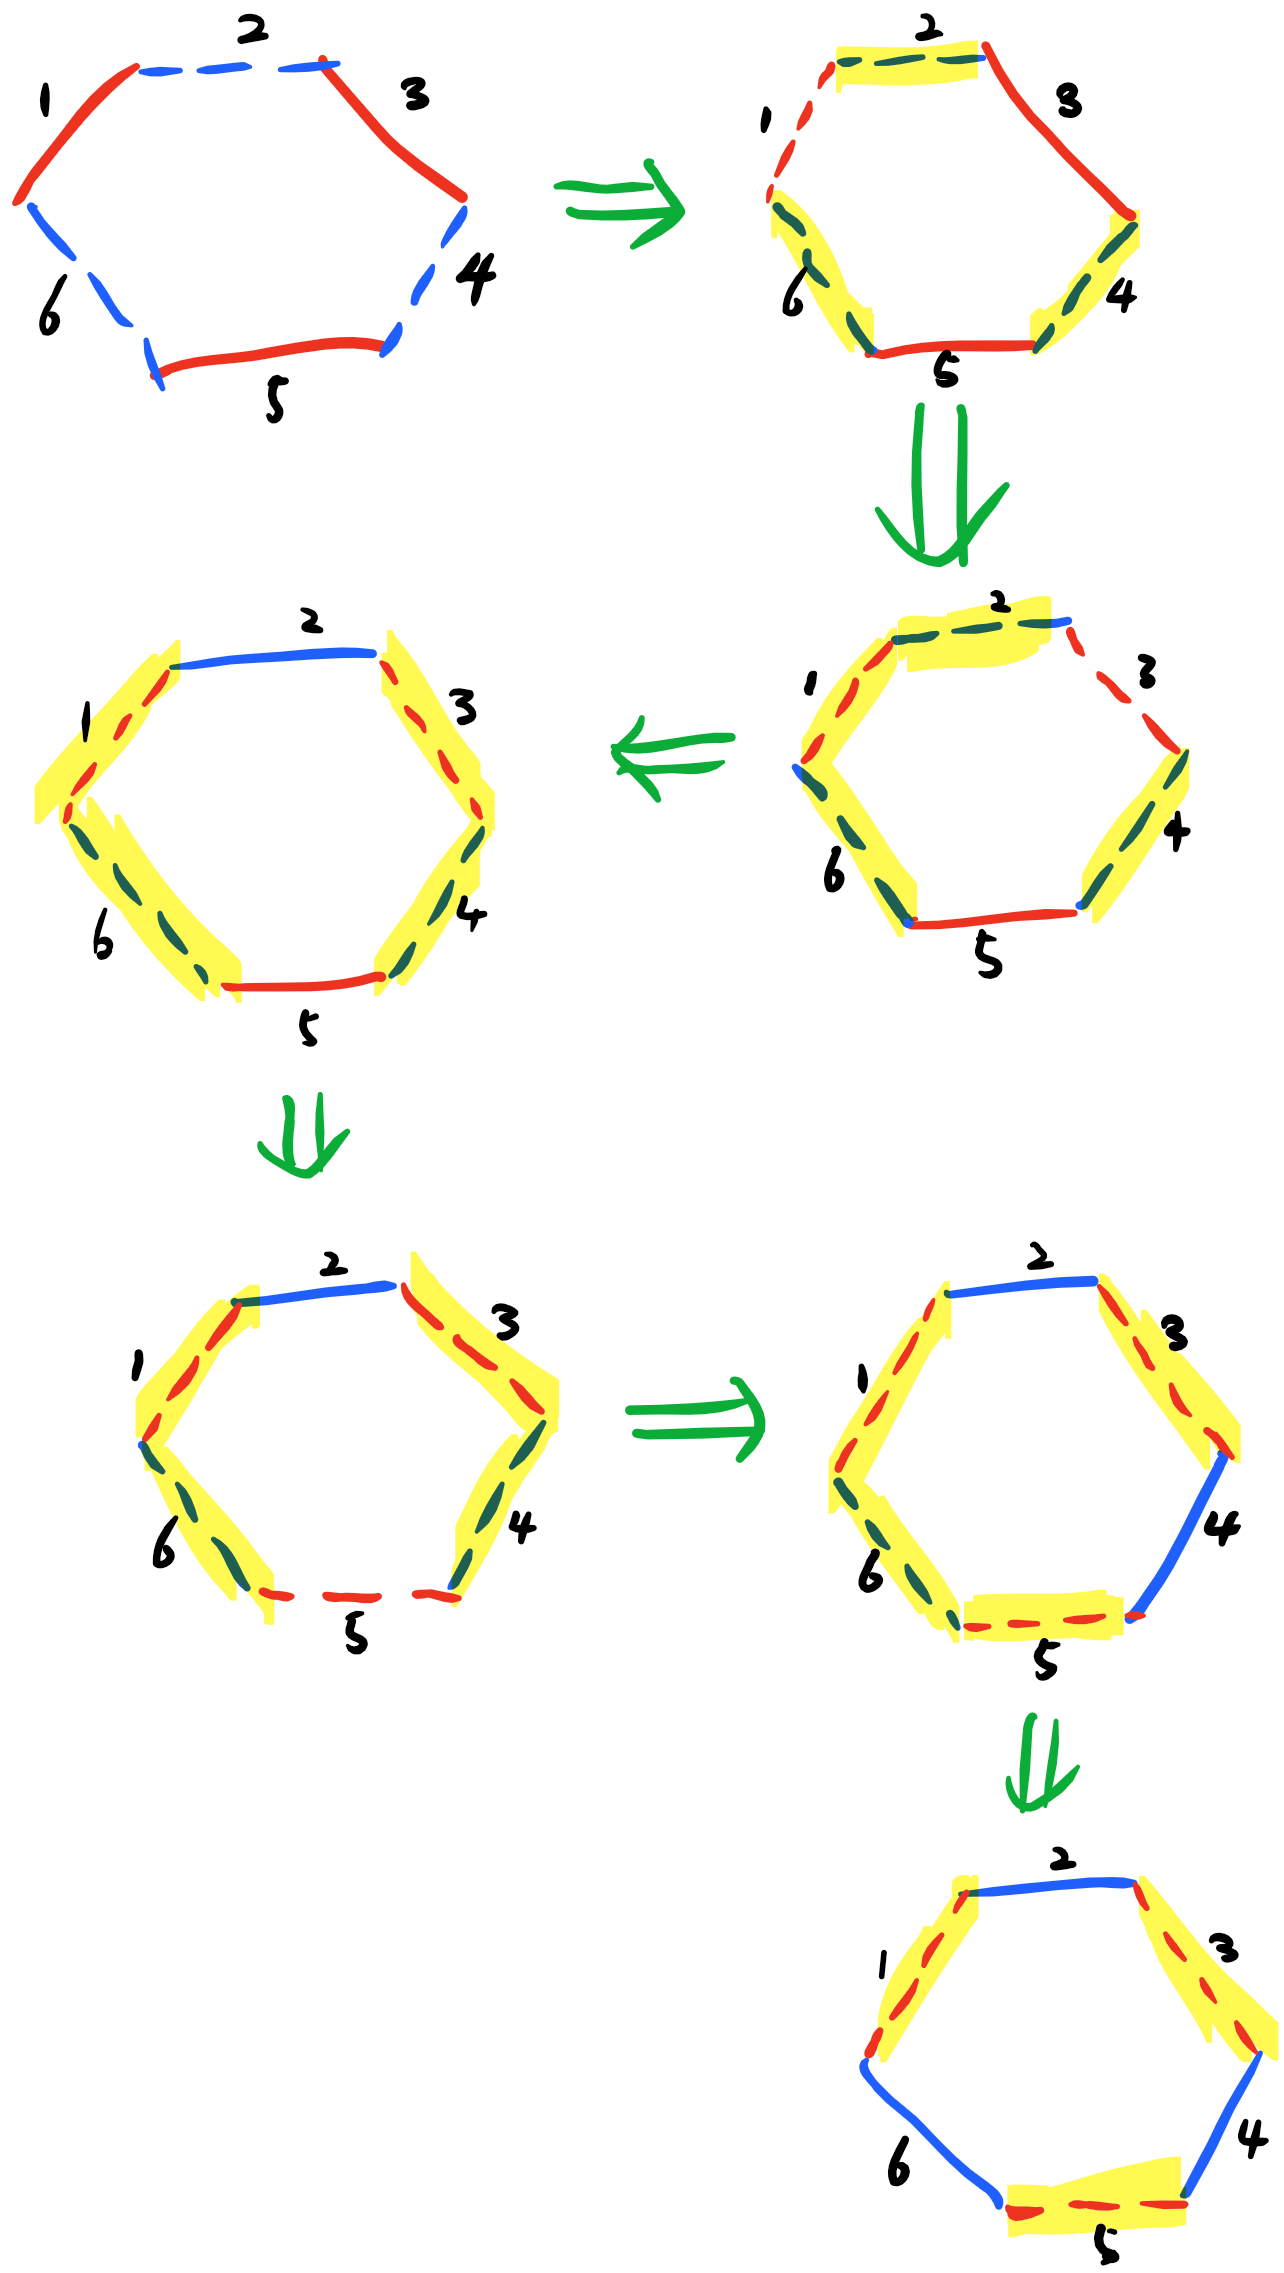
\includegraphics[width=300pt]{pic4.png}
	\caption*{loop to matching}
	\end{figure}

	\begin{figure}[H]
	\centering
	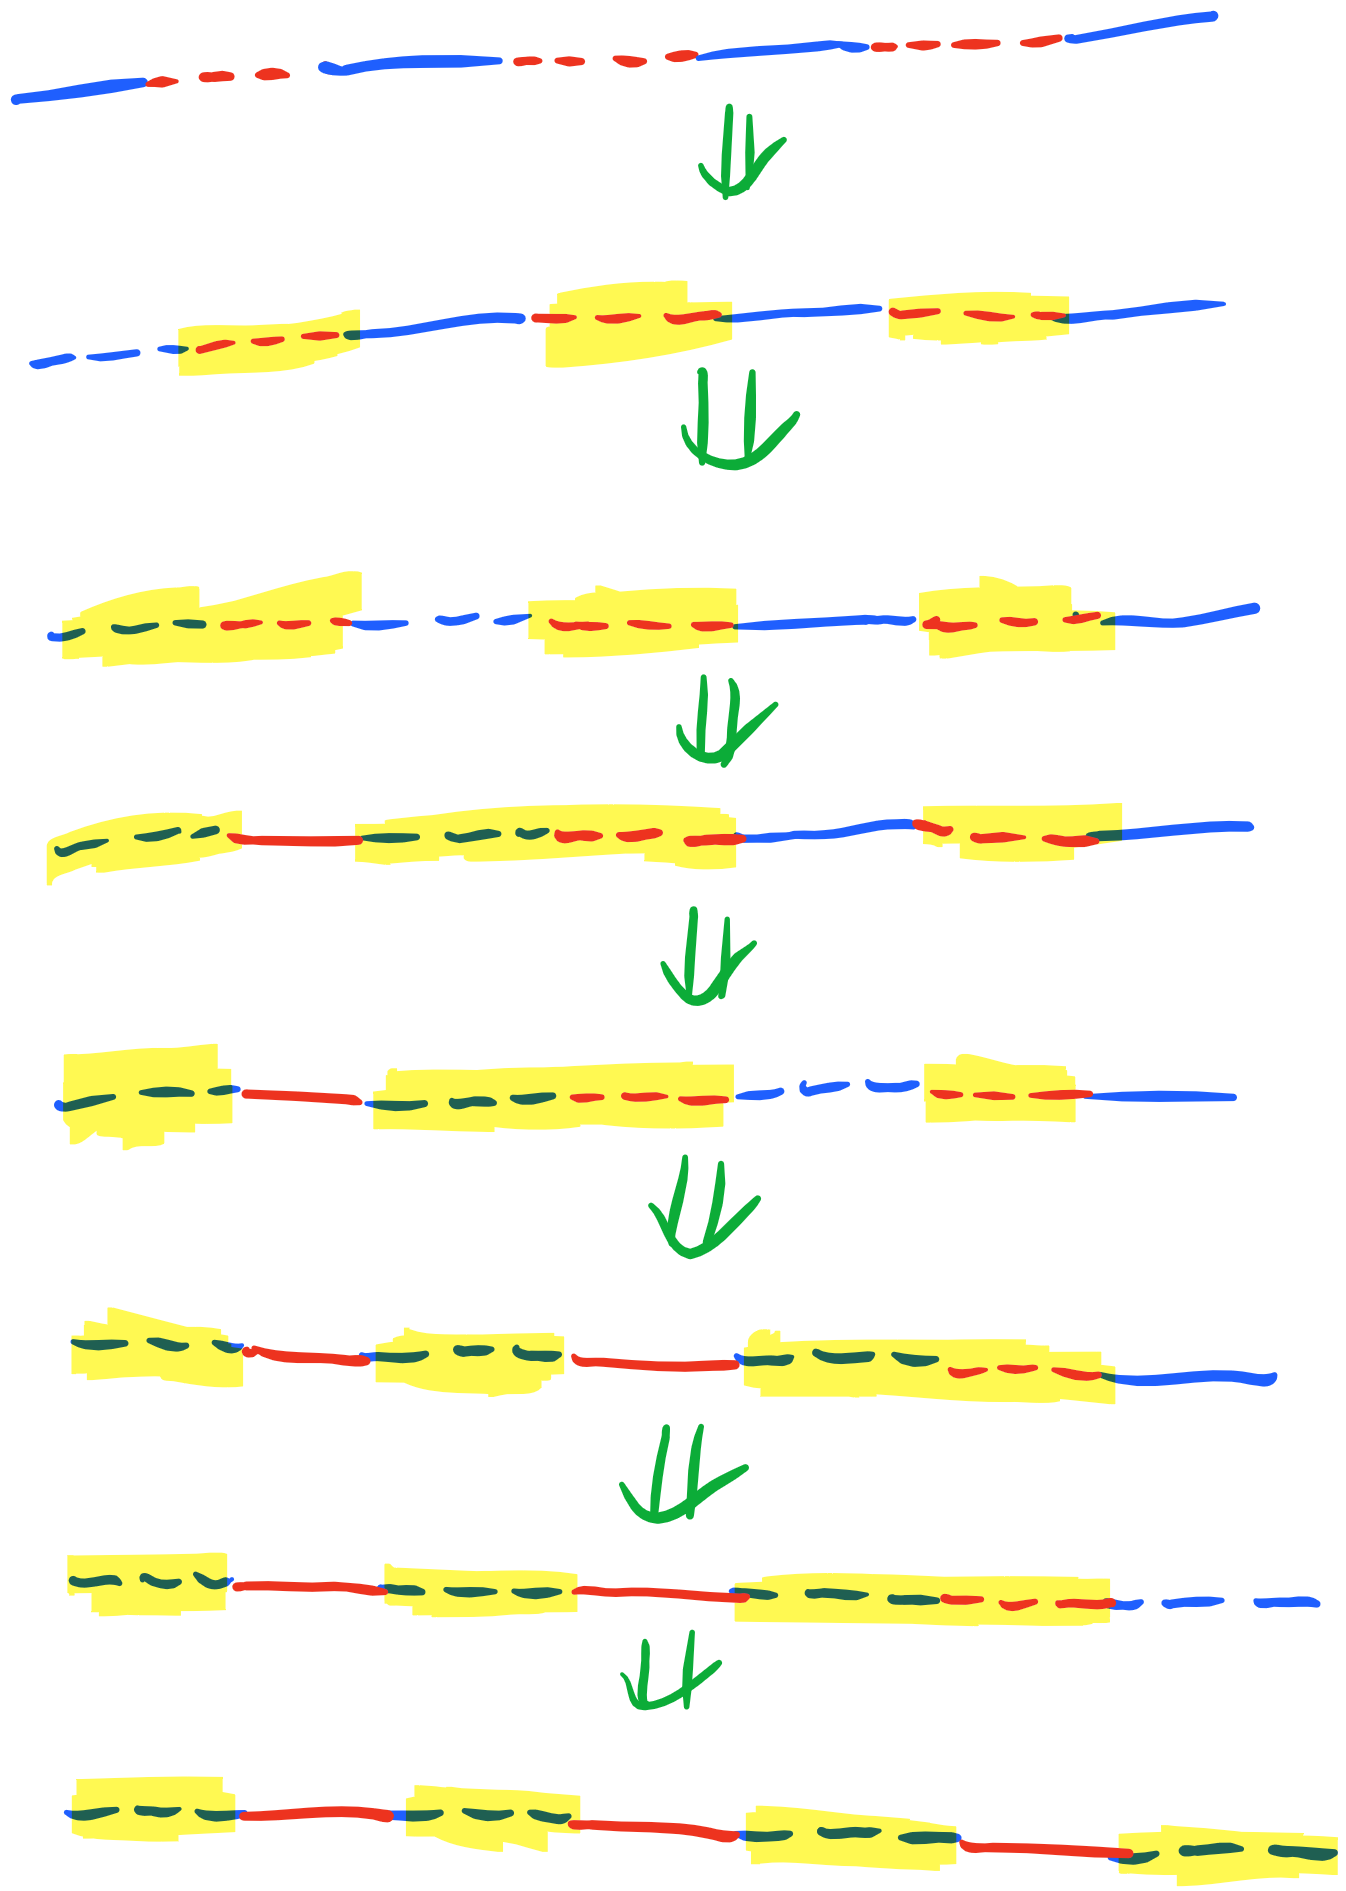
\includegraphics[width=300pt]{pic5.png}
	\caption*{path to matching}
	\end{figure}

	所以我们需要做一些修改:
	\begin{enumerate}
	 	\item 
	 	注意到, loop在去掉一条边之后与path的操作是类似的, 所以我们去掉$I$中编号最小的边.
	 	\item
		注意到, path上会存在有两个相邻边同时被选的情况, 此时我们只选择编号最小的那一个, 这样就将$(I,F)$映射到了一个matching.
	\end{enumerate} 
	
	但是这并不是一个单射, 所以我们需要记录一些信息, 对于修改(2), 我们记录丢弃的那一条边的唯一编号. 对于修改(1), 注意去掉这条边之后我们无法判断当前所在component是一个loop还是一个path, 因此用一个bit来记录这个信息(0: loop, 1: path, etc.).

	因此我们得到了一个$(I, F)\rightarrow\left(\textrm{matching}, E, \{0, 1\}\right)$的单射, 有

	$$P_{IF} \leq 2\Omega\times |E|= O(m\cdot\Omega)$$

	$$\rho = \max_{M,M'}\frac{2m
		\left| \left\{
		(I,F) \mid (M,M')\in \gamma_{IF}
		\right\} \right|
		}{|\Omega|} = O(m^2) \in \textit{poly}(n) $$

	$$\tau(\epsilon) \leq 4\left(\log N + 2 \log \frac{1}{2 \epsilon}\right)\cdot \textit{poly}(n) \in \left(\log |\Omega|\right)^{O(1)}$$
	因此这个\textit{Markov Chain}是\textit{rapidly mixing}的.

\section*{Acknowledgement}
感谢游宇榕提供了一份讲述sample matching的带详细动画的PDF(by Ivona Bez\'akov\'a), 让我理解了带exchange版本的\textit{rapid mixing}推导过程.
\end{document}